\chapter{Development of Medication Tracking Application}
\label{Kap3}

%talking about platforms in general, to get a common understanding 
\section{Used platforms and technologies} \label{platforms}

This chapter focusses on explaining the used technologies and frameworks for developping the mobile RFID application. In the following, the framework 'Nativescript' which can be used for native mobile development will be explained. After that, a further section will discuss the technology of NoSQL and will compare it to SQL database technology. This section will also depict MongoDB, a document store. Finally, the Impinj RFID reader will be presented. In the last section \pageref{app_development} of this chapter the challenges as well as the user scenarios will be shown. 

\subsection{Native Development with NativeScript} 

There exist several ways to create a mobile application. But the challenge is to develop a consistent solution for the existing systems, like e.g. Android or iOS.
To face the challenge of developing a hybride solution which can be run both on Android and iOS devices, Nativescript has been established in the last years \cite{nativescript}. The free and open source technology enables developers to easily build cross-platform native apps with either Javascript, Nativescript or by using Angular \cite{nativescript}. 
Regarding its design philosophy, Nativescript was designed to be approachable to developers from various backgrounds \cite{nativescript}. Moreover, it was designed to be both performant and giving access to native APIs, such as Android or iOS.
The figure \ref{fig:nsarchitecture} gives an impression of the general architecture of Nativescript applications. When developing such applications, one of the given frameworks can be used (e.g. '\{N\} Core', Angular or Vue). Additionally, several Nativescript plugins can be selected. Below the 'NativeScript Core Modules', there are located the 'NativeScript Runtimes' which have direct access to the Native system. By running several commands on the NativeScript \ac{CLI}, the developed Nativescript application can be executed on any physically connected device as well as on the installed emulator or in the cloud. 

\begin{figure}
\centering
\includegraphics[width=\textwidth]{ns_architecture} 
\caption{\label{fig:nsarchitecture}The architecture of NativeScript Applications, adopted from \cite{nsarchitecture}} 
\end{figure}

NativeScript applications can also be developed, built and run on the 'NativeScript Playground' \cite{nsplayground} which enables independent development. Moreover, NativeScript Playground is easier to handle because the development machine does not have to be prepared. Generally, by offering a user-friendly surface, NativSscript Playground is appropriate for beginners who start developing native mobile application.

\paragraph{NativeScript Application Logic}

\begin{figure}
\centering
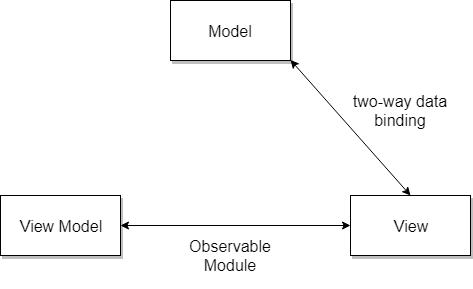
\includegraphics[width=\textwidth]{mvvm_ns} 
\caption{\label{fig:mvvm}The MVVM application logic, adopted from \cite{nativescript}} 
\end{figure}

Nativescript has a \ac{MVVM} application logic (see figure \ref{fig:mvvm}). In contrast to the popular \ac{MVC} application model, Nativescript offers two-way data binding by using the 'Viewmodel' \cite{nativescript}. In every NativeScript application, the model defines and represents data. After that, the data are bound to the view which represents them in a XML file. The 'ViewModel' contains the application logic and exposes all data to the view. Between Model and View, data can either be bound as one-way (default setting, the target property updates when a change in the source property occurs) or two-way data binding (all changes in the directions target-source and source-target will be transmitted). To enable the two-way data binding (see figure \ref{fig:mvvm}), the NativeScript Observable Module has to be implemented. 
In the NativeScript Documentation \cite{nativescript} declares the model files as 'Code Behind' because they have the same name as the view file and are written in Javascript or Typescript. By adding attributes to any XML element in the view file, methods can be implemented in the related model file (in Javascript). 

\subsubsection{NativeScript Sidekick} \label{Native}

Nativescript Sidekick is a solution to run the developed application on unsupported platforms in the cloud. It uses both the local build infrastructure and the cloud build service. Nativescript Sidekick offers users to develop with the provided starter templates, to use verified plugins and to build the app in the cloud. Furthermore, Nativescript Sidekick enables developers to debug, test and refactor their application. 
To search for plugins and to manage these, developers can use the Nativescript Marketplace \cite{nsmarket}.

\subsection{Technology of NoSQL} \label{nosql}

There are many possibilities to store data from application systems. \ac{SQL} can be seen as one of the fundamental database technologies used since the 1980/1990ies \cite[p.137 ff.]{nosql_meier}. The technology of SQL offers advantages, such as consistency, security and integrity of data, as well as the protection of transactions. On the other side, there come along many disadvantages while using SQL. To give an example, checking the integrity of data in case of a higher amount of data implicates the need of a higher processing power. Furthermore, facing large-scale development, the efficiency and performance of SQL based systems are decreasing. Moreover, the flexibility and data handling demonstrates another challenge when using SQL. Actually, in practice, the performance is often more important than the consistency, e.g. in social media.    

In addition to that, many companies are missing clear concepts of architecture as well as migration strategies for the optimal application of  'post-relational databases'. To make SQL databases more flexible and to solve the above mentioned problems, Meier and Kaufmann discuss 'post-relational databases' \cite[p.187 ff.]{nosql_meier}. These databases provide on the one hand partial extensions to relational database systems, on the other hand they offer complete new concepts and methods. To give an example, Meier and Kaufmann talk about decentral or federated databases which imply that the data is distributed on different locally seperated computers \cite[p.188 ff.]{nosql_meier}. By replicating the whole data pool and fragmenting it into different smaller parts which are distributed on several computers, decentral databases raise the data volume effectively. The fragments are called 'shards' and the concept of fragmentation is called sharding or partitioning \cite[p.188 ff.]{nosql_meier}. By using decentral databases, users only have to consider the logical view of data and not the physical fragments, all operations on the database will be driven by the database system.  
Alongside the decentral databases there are also introduced other 'post-relational databases', such as 'Temporal databases', 'Multi-dimensional databases', 'Object-relational databases', 'Knowledge/deductive databases' and 'Fuzzy databases'.

However, there were some NoSQL database technologies coming up in the past ten years. In 2000, these databases were called 'Web-Scale-Databases' because of the need of data storage systems which should handle with the large amount of data of web services \cite[p.221 ff.]{nosql_meier}.
The term NoSQL can be understood as 'Not only SQL' which signifies extension of the existing SQL functionalities. Some data specialists prefer the context of 'no relational databases' which is controversial because of the use of graph databases which deal with relations between nodes.   
In the next section, some examples for the NoSQL data management will be explained and compared to the usual SQL data management. According to Meier and Kaufmann \cite[p.3 ff.]{nosql_meier}, SQL databases are formed on a relation-based model which contains tables with entries. Furthermore, each entry has attributes which are defined by a validating range. A table is defined by its table name, the attribute's name and an identification key. It can have both a column or row order or none of these. The relational model indicates that every table is a set of random tuples and that the relations between data is realized by using tables. The result of SQL queries are always tables which can be uniquely, minimally identified by their identification or primary key.

In contrast to that, the technology of NoSQL offers more possibilities to store data, like for example in key-value stores, column stores, document stores or graph databases \cite[p.16 ff.]{nosql_meier}. These four types of NoSQL databases are also called 'Core-NoSQL-Models'. Besides, other NoSQL database models like object databases, \ac{XML} databases or grid databases are defined as 'Soft NoSQL Models'. 
To give some examples of the 'Core-NoSQL-Models', their fundamental characteristics will be described in the following. The key-value stores (e.g. Cassandra) provide the simplest way to store data by using an identification key and a list of values. Document stores (like e.g. MongoDB \pageref{mongodb}) store the data in form of structured text data like \ac{JSON} or XML. In contrast to key-value stores, document stores have a pre-defined structure but are schema-free which means that the data structure can be changed over the time. Graph databases (e.g. Neo4J) introduce a new way to store data: It introduces a graph-based model. Each graph consists of nodes and edges which connect the edges and demonstrate their relations. Each node can have concepts and object. Both, nodes and edges have a label and can contain properties. Each property contains an attribute and a value. The query language for graph databases is called 'Cypher' \cite[p.16 ff.]{nosql_meier} which is a declarative language. Users of Neo4J and other graph databases are able to specify their retrieval query by defining nodes and edges. By evaluating all possible paths (or connections between nodes and edges), the database system calculates all requested patterns.   
Generally, NoSQL technologies are popular for their high availability as well as their protection against system failures by using different replication concepts, e.g. 'Consistent Hashing' \cite[p.11 ff.]{nosql_meier}. In addition, NoSQL is characterized by its vertical and horizontal aligned scalability, its weak or non-existent restrictions concerning schemas and data models. Along, NoSQL databases offers simple data replication and easy access through API \cite[p.221 ff.]{nosql_meier}.  
Edward and Sabharwal discuss the pro and cons of NoSQL technologies in their book \cite[p.17 ff.]{mongodb_edward} which will be given in the next paragraph.
One the one hand, NoSQL offers high scalability, manageability and administration (such as automated repairs, distributed data etc.), low cost and flexible data models. But on the other hand, using NoSQL factors like maturity, limited query capabilities, administration (installing and maintaining solutions) and limited expertise (developer and administrator community are limited).

\paragraph{Document Stores} \label{documentstore}

In the last section, there were introduced some examples of NoSQL databases. This paragraph reveals with the characteristics, advantages and disadvantages of document stores because the deployed database, MongoDB, is a document store. 
Basically, document stores consists of databases, containing collections with documents. Each document can have its own internal structure and is defined by JSON-like files which look like a list of attribute-value-pairs. As a 
On the one hand, like key-value-stores, document stores are schemafree so that users do not have to define a schema for the database. Nevertheless, document stores offer the possibility of structuring the stored data. In addition to that, the structured data will be stored as records which are called documents. Generally, document stored were developed for web services. Thus, they are easily integrable with JavaScript and \ac{HTTP} and easy horizontally scalable. 
On the other hand, as a disadvantage, document stores do not support referential integrity either normalization.
Nevertheless, because of being schemafree, document stores propose high flexibility to store different data (see section Excursus: BIG DATA \pageref{bigdata}). Referring to the flexibility, fragmentation and sharding of an existing data pool can be seen like that. In excess of relations between data, documents do not have any relation to each other but each document contains a closed collection of data in which familiar data can be linked.

\paragraph{Queries (Map and Reduce)}

Document stores are exceptional in that they query in a Map/Reduce procedure which enables the possibility of querying parallel and accelerated. Consecutive, the Map/Reduce procedure will be explained briefly. 
To begin with, the method can be divided into two phases: During the first phase (Map, 'group by'-phase), the data is grouped by criteria. This is realized by a Map-function which asociates for each document an appropriate specific processing by establishing an index (= map) and sending it back. A map can be compared to an associative array with one or multiple key-value-pairs per document.  
After that, in the second phase (Reduce, 'Aggregation'), a Reduce-function (can be compared to SQL statements) returns for each key in the index a row of the Map-Function and aggregates their related values. This second phase is optional.

\paragraph{CAP theorem} \label{CAP}

The \ac{CAP} theorem \cite[p.15 ff.]{mongodb_edward} also known under the name of  'Brewer's Theorem', was developed Eric Brewer in 2000. It describes three important characteristics of a NoSQL database system: Consistency refers to all data which has to remain consistently after every operation. Availability means that the system itself has to be available at any time. Partition tolerance states that every system is working even if is partitioned into groups of independent servers \cite[p.15 ff.]{mongodb_edward}.

\paragraph{ACID vs. BASE}

Concerning the topic of transactions in SQL, Meier and Kaufmann \cite[p.136 ff.]{nosql_meier} mention the \ac{ACID} principle. Atomacity means that a transaction is either performed completely or not. Consistency refers to transactions which cause conviction from one state into another. At this point, Meier and Kaufmann declare a transaction as 'an unit to obtain consistency'. Isolation signifies parallelly run transactions which will produce the same results as single-user environments becaue each transaction is run isolated. The Isolation principle includes the protection from unwanted side-effects. When talking about the isolation of transactions, they can be called 'unit of serializability'. The last principle, durability refers to the different states of databases which have to be maintained until the next transaction. In that case, every transaction can be seen as 'unit of recovery'.

The \ac{BASE} principle which refers to NoSQL technologies says that a consistent state in a distributed database system can take place retartedly. Based on the CAP theorem \pageref{CAP}, BASE signifies that the system is always available and that all states in the systems are soft which means that even if there is no input provided to the system, the state will be changed over time \cite[p.15 ff.]{mongodb_edward}. The last feature of BASE stands for eventually consistency which means that the system will attain consistency in long run provided no input is sent.

When comparing both ACID and BASE, apparently there exist many parallels. 'Atomacity' can be compared to 'Basically Available', 'Consistency' to 'Eventually Consistency', 'Isolation' to 'Soft State'. But one criteria of ACID is not realized within BASE: Durability \cite[p.1 ff.]{mongodb_edward}.

\subsubsection{Characteristics of NoSQL Databases}

A \ac{DBMS} defines a software which describes, stores, queries data independently from an application \cite[p.2 ff.]{nosql_meier}. It consists both of a storing and managing component. The storing component is composed of all data which has to be stored in organizational form and their description. The managing component contains a querying or manipulating language to evaluate data and to change them, such as access control units and an user interface. When it comes to the use of web applications and a heterogeneous data pool in real-time, SQL databases are often not suitable for these problems. In this case, a NoSQL database should be considered. 

\subsubsection{Excursus: BIG DATA} \label{bigdata}

The following section shall only act as additional contextual knowledge paragraph. 
The term 'Big Data' has been emerged during the past 10 years. Due to the enormous data pool, e.g. in social networks or user analysis, which is not easy to manage with usual software tools, new data technologies were needed. As a solution, NoSQL technologies have been arised. Furthermore, Big Data refers to unstructured data which comes from different sources \cite{nosql_meier}. 
Edward and Sabharwal define Big Data as the following: It is a '[...] term used to describe data that has massive volume, comes in a variety of structures and is generated at high velocity. This kind of data poses challenges to the tradtitional \ac{RDBMS} used for storing and processing data. Big Data is paving way for newer approaches of processing and storing data.[...]' \cite[p.1 ff.]{mongodb_edward}. Furthermore, Edward and Sabharwal refer to an explosion of data created by smartphones, social networking sites, in short words from various sources in various formats, such as video, text, speech, log files and images. The type of stored data varies by its 'sector', e.g. retail and whole sale, administrative parts of government, financial services mainly generate text or numerical data (including customer data and transaction information). On the other hand, in the healthcare, manufacturing, media and communication sector especially multimedia as well as image data is produced. To give an example, X-Rays, CT and other scans dominate the storage volumes in healthcare. 
Another important point, when it comes to large amounts of data is the consumation model or the various sources from which data is produced and subsequently consumed \cite[p.6 ff.]{mongodb_edward}. Edward and Sabharwal declare two models: In the old model, few companies produced data and all others (users, clients, etc.) consumed them. But nowadays, they claim that '[...] all of us produce data and all of us consume them [...]' \cite[p.6 ff.]{mongodb_edward}. This creates a new challenge of developing multiple user data models and make the existing data management system more scalable than in the past. 

\paragraph{Velocity, Variety, Volume}

When talking about Big Data, often there come up three descriptive terms: Velocity, Variety and Volume.
Velocity refers to the real-time high-speed evaluation of the upcoming data \cite{nosql_meier},  also known as 'real-time insight' \cite{mongodb_edward}. Edward and Sabharwal describe velocity as 'Data in motion' \cite[p.7 ff.]{mongodb_edward}. Besides, they mention that if data cannot be processed at required speed, it losses its significance. For many companies and organizations, it is very important to process data both when it is moving as well as when it is static. 
Variety means that there are distinct formats of data: structured (e.g. integer, string), semi-structured and unstructured data \cite{nosql_meier}. Edward and Sabharwal describe variety as 'Data in many forms' \cite[p.7 ff.]{mongodb_edward}. As mentioned in the last paragraph, data can vary from simple text files, log files, streaming videos, photos, meter readings, stock ticker data, PDFs and many other unstructured format.   
The last characteristic of Big Data, volume, deals with the high amount of data \cite{nosql_meier}. Edward and Sabharwal describe volume as 'Data in many forms' \cite[p.7 ff.]{mongodb_edward}. They see a reason for the higher volume in businesses becoming more transaction-oriented and the number of transactions is increasing. Moreover, more devices are connected to the internet which increases the size of data.
Calolas et al. refer to challenges like e.g. dealing with tremendious amounts of data, unstructured data (diversity of \ac{OSN}) as well as the complexity to challenge analyzing social networks data \cites{trends_nosql}.

\paragraph{Usage of Big Data}

Edward and Sabharwal depict five large use cases of Big Data which will be explained in the following \cite[p.9 ff.]{mongodb_edward}. Firstly, visibility of data is very important for many companies. For example if data is accessible across departments of a company, it can be readily integrated. This reduces the search and processing time, improves product quality according to present needs \cite[p.9 ff.]{mongodb_edward}. Secondly, discover and analysis information is another use case for large amounts of data. After capturing detailed data, e.g. of inventories, employees or customers, new information or patterns will be discovered and analyzed. The captured information and knowledge can be used to improve processes and performance of companies \cite[p.9 ff.]{mongodb_edward}. Thirdly, segmentation and customizations can be effected by means of using Big Data. To give an example, the segmentation of customers is based on various parameters and can aid in targeted marketing campaigns or tailoring of products to suit the needs of customers \cite[p.9 ff.]{mongodb_edward}. Fourthly, Big Data can aid, improve or automize decision making by using Big Data analytics which can minimize risks and uncover valuable insights. Lastly, Big Data can strengthen innovations in existing products by using data gathered for actual products \cite[p.9 ff.]{mongodb_edward}.    

\paragraph{Big Data challenges}

The issue 'Big Data' not only offers many possibilities or use cases, but also faces many challenges \cite[p.11 ff.]{mongodb_edward} which will be discussed in the consecutive paragraph. To start with, Edward and Sabharwal indicate policies and procedures which can constrain the use of Big Data. They refer to data privacy, security, intellectual property of organizations. Furthermore, in order to comply with various statutory and legal requirements, Big Data has to face the challenge of data handling, which includes issues around ownership and liabilities around data. In second place, the access to data has to be controlled precisely. Since some data might be available to third parties, the gaining access poses a legal, contractual challenge. After that, in order to handle Big Data, new tools as well as technologies have to be built specifically. Moreover, there might exist legacy systems in several organizations or companies which have to deal with Big Data. Besides, there exists a lack of experienced resources in these newer technologies which is also a challenge to.
Most of the legacy systems are designed to work with structured data \cite[p.11 ff.]{mongodb_edward}. Since legacy systems are created to perform fast queries and analysis on tables and columns, they cannot be used to hold or process Big Data (which contains unstructured data). Another important point is the data storage for Big Data. Currently, in many companies, data is stored on big servers (using \ac{NAS} or \ac{SAN} systems) \cite[p.11 ff.]{mongodb_edward}. With the increasing data, the server size and backend storage size has to be increased. 
Lastly, when handling with Big Data, data processing is very important . Usual algorithms in legacy systems are designed to work with structured data and are limited by data size. Therefore, legacy systems are not capable of handling processing of unstructured data, high volumes of data, speed etc. To capture value from Big Data, the deployment of newer technologies are needed. 

\paragraph{Big Data technologies}

Edward and Sabharwal propose several ways of implementing Big Data technologies \cite[p.12 ff.]{mongodb_edward} which will be depicted in this paragraph. To begin with, Big Data needs new storage and processing technologies which are designed for large, unstructured data. After that, other technologies like parallel processing, clustering are emerging in order to handle Big Data. Additionally, large grid environments, high connectivity and high throughput offer new fields for software developer and data scientists. Finally, cloud computing and scale-out architectures have been arised during the last years.

\subsubsection{Use case of NoSQL Databases: 'Socii System'}

To give an example of the use of NoSQL technologies, the next section will focus on explaining a developed system 'Socii'. 'Socii' was developed from Jroge Daniel Calolas, Alda Lopes Gancarski and Pedro Rangel Henriques. In their article 'Online Social Network Analysis Visualization Using Socii' \cite[p.218-228]{trends_nosql}, they describe the several technological challenges they faced during development but also the benefit of this social network analysis and its scientific importance. In short words, 'Socii' is a system which enables the analysis and visualisation of social networks by helping \ac{OSN} users to exploit and understand their own networks through a user friednly interface. During development, Calolas et al. were facing four main principles: simplicity, accessibility, OSN integration and contextual analysis.
One big problem before developing of 'Socii', Calolas et al. mention was the observation of social structures and the analysis of these networks. By establishing 'Socii', the authors Calolas et al. wanted to proprose to fill the gap or struggle that OSN users have in understanding their network. To give an example of these struggles, there were three main topics, Calolas et al. were facing: 'how relationships evolve along the time', 'what role play these friendships within the network' and 'how they can analyze and visualize their networks based on social properties (such as mutual relationships, geographical positions, personal tastes and preferences or hobbies)' \cite{trends_nosql}. 

\paragraph{Structure and flow of data analysis and visualization systems}

When introducing 'Socii' as an social analysis tool, Calolas et al. also talk about several tasks and steps during the process of data analysis and visualization systems. Firstly, data has to be extracted (through APIs, web crawlers and web scrapper. Secondly, data is achieved which requires careful selection of relevant data to store \cite{trends_nosql}. In order to have an efficient system that provides good structure for data analysis, one needs to select the data carefully. In the third step, data is explored by defining of what one user wants to do with the data. Furthermore, during this step, there are two important questions: What are the applications that can be seen for the stored data? How can the system digest and transform data in order to make it useful and interesting for the end user? 
Lastly, in the fourth step, data is visualized which means the kind of presentating or showing the transformed data is chosen by the user. Particularly, the work of the data scientist has a huge impact on the end user. In generals, the data visualization targets a general audience.  
By extension, 'Socii' affirms web availability, OSN's  integration, contextual analysis and being a trade-off for such gains the system performance.

\paragraph{Main functionalities of 'Socii'}

One of the main functionalities of 'Socii' is information extraction and data mining \cite[p.223]{trends_nosql}. These include extracting some user networks form given OSNs by calling web crawler modules which then return the extracted information. After that, an extraction manager sends the extracted data through a simple data mining process in order to data normalized before it is stored in the database (MongoDB). Web crawlers are implemented in Python and the crawling operations are performed using XPath selectors to extract the information that are needed to build the network.
Generally, the main functionalities of 'Socii' amount to OSN contextual netowrk analysis (with relatively low complexity) \cite[p.227]{trends_nosql}. Moreover, 'Socii' intends to integrate data from different OSNs by processing a set of node properties displayed together with the network structure. Roughly, Calolas et al. implemented three features of 'Socii'. To start with, 'configurable, parameterized analysis' enables users to select several metrics upon a given network. Consequently, 'clear, intuitive social graph visualization and interaction' refers to the visual web component of 'Socii' which provides users a set of visual features (coloring, node discovery etc.). Thirdly, 'Socii' offers an 'organized overview upon SNAs and OSN data' which include visual components that aggregate SNAs metrics and OSNs information. Thus, users are able to cross information from both and can derive conclusions from intersecting the information \cite{trends_nosql}. 

\paragraph{Limitations of 'Socii'}

As shown in the last paragraph, 'Socii' offers many features to analyse Big Data especially in social networks. Nevertheless, Calolas et al. depict some limitations and disadvantages which will be explained in the following. 
First of all, there exists a technical and architectural struggle of feeding the system through an extraction pipeline built on top of the web crawlers. This is known and proved by a very slow, limited and error-prone method for data extraction and the authors call it the 'bottleneck' of their built system \cite [p.227]{trends_nosql}. 

\paragraph{Future outlook of 'Socii'}

According to Calolas et al., 'Socii's implementation should be completed to work with other OSN's. Furthermore, it can be extended to perform evaluation and validation of system with users having accounts in several OSNs and several profiles. 

\subsubsection{NoSQL Technology: MongoDB}\label{mongodb}

As mentioned in section Document Store \pageref{documentstore}, this type of NoSQL database provides high availability, scalability and partitioning options \cite[p.25 ff.]{mongodb_edward}. Nevertheless, there are some disavantages when using MongoDB or any other document stores: For instance, both consistency and transactions are not supported. 
In contrast to relational databases, MongoDB does not consist of tables and rows, but of collections containing documents which make it both flexible and scalable \cite[p.25 ff.]{mongodb_edward}. Collections can be compared to tables in SQL but are schemaless. Instead of having one unique schema within the same collection, every document can have its own set of fields, and common fields can store different values across documents.  
All data is stored in \ac{BSON} documents which assures that related data is placed all together in one place. BSON documents are JSON documents in binary-encoded format. It is the extended form of the JSON data model and is fast, high traversible and lightweight \cite[p.31 ff.]{mongodb_edward}. Moreover, JSON/BSON documents contain schema-less models. Each documents stores data as key-value pairs, where the value can be left blank (see above, disadvantage of consistency). Thus, users of MongoDB have to ensure and check the consistency of their data when adding new data.

One characteristic of MongoDB is the _ID (key) which can be compared to the label or name of a colum in RDBMS. If not explicitely specified by the user, a unique value is automatically generated and assigned  to it by MongoDB. Basically, the key value is immutable and can be of any data type except arrays \cite[p.31 ff.]{mongodb_edward}.
Queries in a MongoDB database use the keys (_ID) in documents which makes it possible to query documents spread across multiple servers. 
MongoDB uses primary-secondary replication, where the primary replication accepts the write requests. To be more precisely, if the write performance needs to be improved, the mechanism of sharding can be used. Sharding means that data will be split across multiple machines which are enabled to update different parts of datasets \cite[p.25 ff.]{mongodb_edward}. Besides, this mechanism is automatic in MongoDB, so that as more machines are added, the data is distributed automatically.

\paragraph{Limitations and possibilities of MongoDB}

There are many advantages and disadvantages, limitatiions and possibilities when using MongoDB. The following paragraph will discuss these and give some examples.

Generally, MongoDB offers many features which MySQL does not. To give an example, MongoDB supports secondary indexes, atomic updates at a per document level. Additionally, queries can be executed by using query documents. Furthermore, MongoDB provides replica sets which are based on master-slave replication with automated failover. After that, MongoDB provides a built-in horizontal scaling. Finally, MongoDB can be run everywhere (e.g. on Cloud, \ac{VM}, servers etc.) because it is written in C++. 

Another feature of MongoDB are 'Capped Collections' which store documents in the inserted order. When the capped collection reaches its storage limit, documents will be deleted from the collection in the inserted order (analogous to \ac{FIFO} principle). Capped collections are often used for log files in order to get these automatically truncated after a certain size. In the end, capped collections guarantee preservation order data in the insertion order \cite[p.31 ff.]{mongodb_edward}.

On the other hand, in contrast to relational databases like MySQL, MongoDB does neither support JOINs nor fully generalized transactions \cite[p.25 ff.]{mongodb_edward}. Secondly, when using MMAPv1 as storage engine, the used space is too large because its data directory files are larger than the database's actual data \cite[p.226 ff.]{mongodb_edward}. For that reason, it is recommended to use MongoDB's WiredTiger storage engine which compresses all files and reduces the storage size by 50\%. Moreover, once a collection is dropped diskspace is automatically reclaimed (unlike MMAPv1 engine).
Thirdly, when using MongoDB BSON documents, their usage is limited the size, nested depth and field limits of the specific document \cite[p.228 ff.]{mongodb_edward}. After that, namespaces as well as indexes are limited, for instance the maximum size of indexed items has to be1024 bytes. The number of indexes per collection must not exceed 64 indexes. Moreover, the usage of sharding is limited \cite[p.230 ff.]{mongodb_edward}. Therefore, if shards were implemented too late, a slowdown of servers is caused because splitting and migration of chunks takes time and resources. Thus, Edward and Sabharwal  recommend to shard a collection before reaching 256 \ac{GB}. 
Next, when using MongoDB, there exist some security limitations because the database does not provide authentication by default. This enables every user which is connected to the database server, to read, change, add and delete data. In addition to that, the connections to and from MongoDB are not encrypted by default. Therefore, when starting the database server on a public network, it is recommended to use encrypted communications. Therefore, Edward and Sabharwal propose the SSL-supported build of MongoDB (which is available as 64-bit version) \cite[p.230 ff.]{mongodb_edward}. What is more, using MongoDB implicates write and read limitations, such as case-sensitive queries and type-sensitive fields since there is no enforced schema \cite[p.231 ff.]{mongodb_edward}. For instance, users have to ensure the correctly used type when adding new data. By the same, replica sets which can be used to ensure data redundancy, are limited by the number of the members in every set. When using such replica set, one member acts as a primary member whereas the rest acts like secondary members (a node needs the majority of votes to become primary).

All in all, MongoDB provides many possibilities but also limitations. Generally, it should be clarified that MongoDB is neither adequate to be used in a highly transactional system nor in business intelligence applications where issue-specific databases shall generate highly optimized queries. Finally, it should not be used in applications requiring complex SQL queries. Instead, it is recommended to store high amounts of data and to ensure its availability at any time. 

\paragraph{MongoDB: Best Practices}

Edward and Sabharwal suggest some 'best practices' when using MongoDB \cite[p.234 ff.]{mongodb_edward} which will be explained briefly in this paragraph. 
First of all, the correct hardware should be chosen. For example, the more internal memory is given, the better the performance of the MongoDB application. Another important point is the CPU: for its productivity, MongoDB needs a fast \ac{CPU} clock speed, as well as a high \ac{RAM}. Moreover, using SATA SSD and \ac{PCI} ensures good price as well as performance results.
Concerning the best practices in coding, Edward and Sabharwal propose to set a correct data model. Further, they recommend avoiding application patterns that lead to unbounded growth of document size as well as to design documents for future which are better to handle with MongoDB's drawback. Besides, documents should be created with an anticipated size where ever applicable. But the most important point when coding is to check data consistency \cite[p.234 ff.]{mongodb_edward}. 
With respect to the data safety and how to provide it in the deployed MongoDB database, Edward and Sabharwal both replication and journaling of data \cite[p.234 ff.]{mongodb_edward}. Furthermore, the repair should be the last resort for recovering data in case of a server crash. Basically, they recommend to always specify a timeout with assuming the command and to run the MongoDB server instance in trusted environment with access control.
Likewise, concerning the administration of MongoDB, Edward and Sabharwal submit to perform instant-in-time backups of durable servers and to use repair in order to compact databases \cite[p.234 ff.]{mongodb_edward}. Correspondingly, managing the replication log is of administrative concern \cite[p.240 ff.]{mongodb_edward}. 
Respecting sharding, it is important to select a good shard key. Moreover, Edward and Sabharwal recommend using three config servers in production deployments to provide redundancy \cite[p.240 ff.]{mongodb_edward}. 
Finally, Edward and Sabharwal introduce 'monitoring' which means that every MongoDB system should be proactively monitored to detect unusual behaviours \cite[p.240 ff.]{mongodb_edward}. To put this into practice, MongoDB's free hosted monitoring service, MongoDB Cloud Manager (which contains a dashboard view of the entire cluster metrics, can be used. Besides, MongoDB itself provides 'mongostat' and 'mongotop' to gain insight into the performance of the database instance (e.g. operation counters, active working sets etc. are shown). 

\subsection{Impinj RFID Lector and Antenna}

The developed system was tested and run on a Speedway R420 RAIN RFID READER \cite{speedway} with four antenna ports (extendable to 32 antennas with an Impinj Antenna Hub \cite{speedway}) and a flexible read range (short and long-range reads are supported). According to the manufacturer's web page \cite{speedway}, the Speedway R420 RAIN RFID READER can be connected to Impinj Autopilot technology which automatically optimizes the reader's operation for its environment. Furthermore, there can be downloaded the appropriate software from the Impinj web page \cite{speedway}.
In the following section, there will be given some information about Impinj, RAIN RFID as well as some example use cases. 

\subsubsection{General Information}

To start with, \ac{RAIN} RFID will be presented. RAIN RFID is a global alliance promoting universoal adoption of UHF RFID technology \cite{rainrfid}. It can be compared to NFC Forum, WiFi Alliance or Bluetooth SIG. Moreover, RAIN RFID uses a GS1 UHF Gen2 Protocol which is ISO-standardized (18000-63). According to the alliance, the term RAIN shall represent the node between UHF RFID and the cloud where RFID-based data can be stored, managed and shared. Several RAIN RFID uses reader to read and write a tagged item, manage data and take action.
Impinj (also known as NASDAQ:PI) enables wireless connection of multiple everyday items, such as apparel, medical supplies, automobile parts, luggage etc. The Impinj platform uses RAIN RFID to deliver timely information about all items to the digital world (application systems) \cite{impinj}.

\subsubsection{Examples}

Impinj mentions some example use cases when implementing the Speedway R420 RAIN RFID READER: Inventory Management, Asset Tracking and enhanced shopper experience. 
The DeRoyal Industries, Inc. which was founded 1973 is a medical device facturer\cite{deroyal}. With the aim of improving clinical quality and economic health of customers, DeRoyal provides surgical devices, unitized delivery systems, orthopedic supports and bracing wound care dressings. One of their software solutions is the system 'DeRoyal Continuum Safe' \cite{deroyal}. By using the Impinj platform and RAIN RFID, DeRoyal Continuum Safe automatically captures and tracks data from medical supplies in the operating room, emergency department and catherterization lab. The solution includes packaging which is tagged with RAIN RFID tags. According to DeRoyal, the system provides many advantages, such as reducing the time staff spend managing supplies so that they can focus more on patient care. Besides, DeRoyal Continuum Safe improves billing accuracy for supplies used during procedures. After that, the likelihood of infections is reduced by ensuring the availability of necessary supplies. Lastly, DeRoyal achieved to provide a data-driven supply chain management \cite{deroyal}. 

%
% talking about application, more details
%
\section{Application development} \label{app_development}

\subsection{Challenges during development}

Mongodb integration within nativescript application 
--> with Node JS package installer 
but synchronization with data from Mongodb was difficult

Real-time synchronization of mobile application with MongoDB server was difficult. Firstly, HTTP Request/Response was implemented to connect the mobile device with the RFID reader and the database. But only one device was enabled to connect to the server. Thus, another solution had to be considered. Finally, a Socket.IO connection was implemented to both server and client. Socket.IO enables two-way data synchronization and cannot be compared to HTTP Request/Response. Furthermore, with Socket.IO, it was possible to run the application on various mobile devices without any complication. 

\subsection{Progress of development}

\subsubsection{User Scenario}

The following two images show the start page and the item information page of the developed application. 



\begin{figure}
\centering
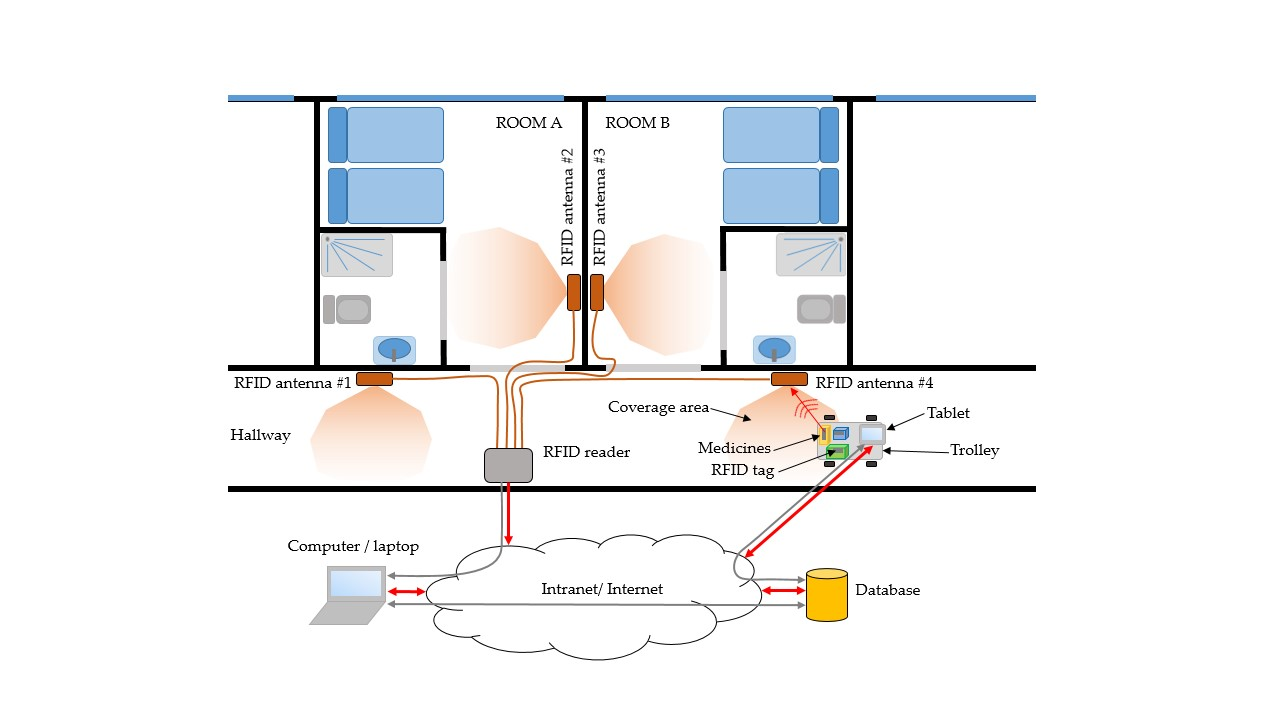
\includegraphics[width=\textwidth]{app_functionality} 
\caption{\label{fig:appfunctionality}Application scenario of RFID application} 
\end{figure}


\begin{figure}
\centering
\subfigure[Start page of application]{\label{fig:a}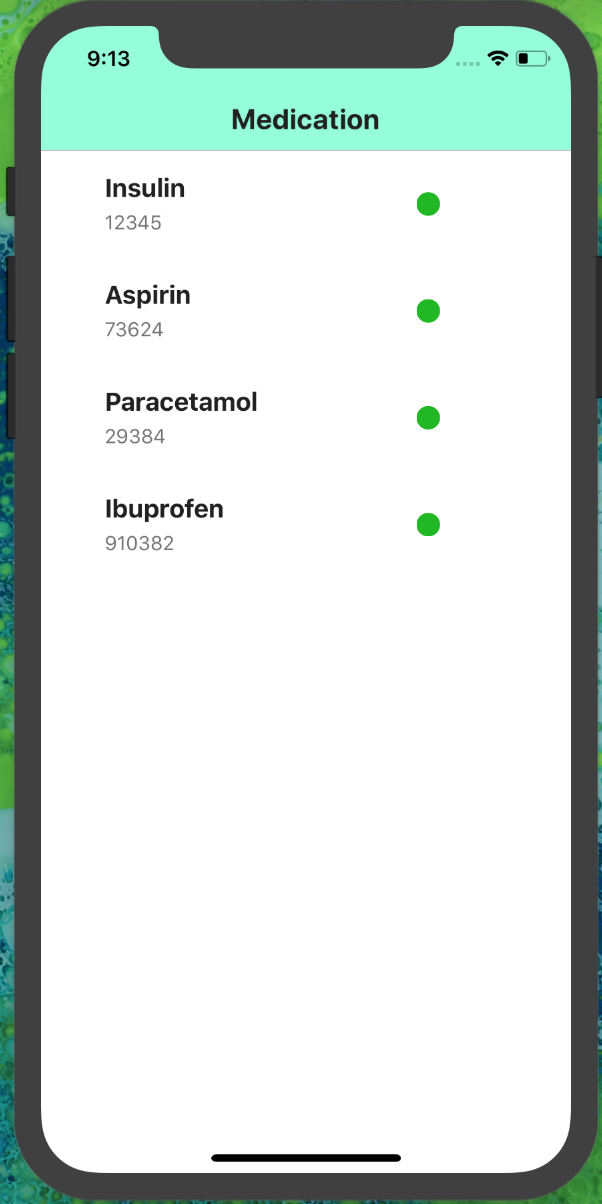
\includegraphics[width=6cm, height=12cm]{Mainview}}
\subfigure[Item information page]{\label{fig:b}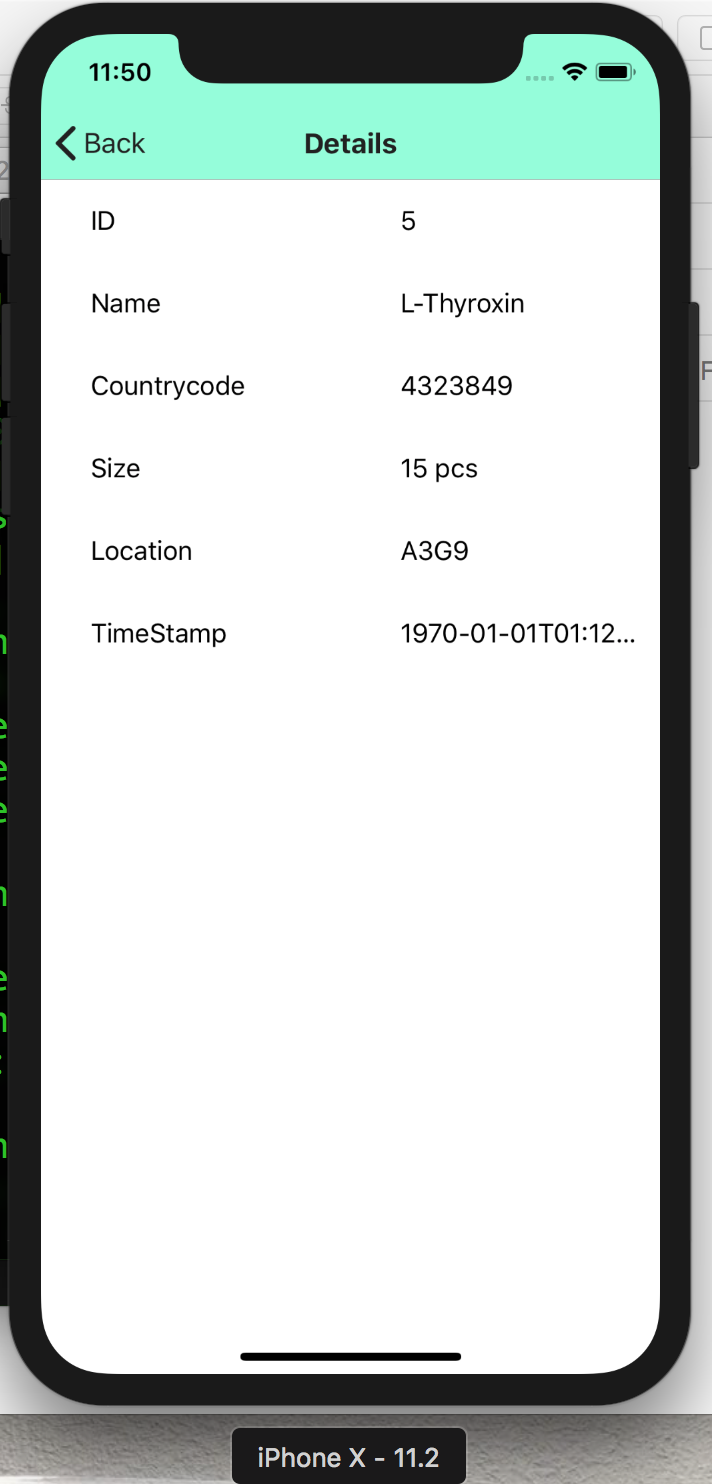
\includegraphics[width=6cm, height=12cm]{Detailview}}
\caption{Layout of application, Screenshot of iOS Simulator}
\end{figure}




\subsubsection{Software Architecture}

\begin{figure}
\centering
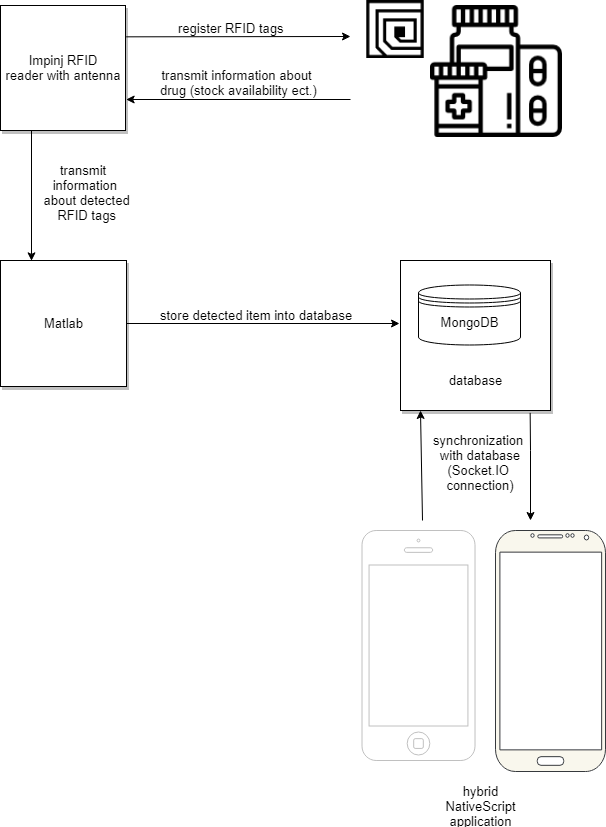
\includegraphics[width=\textwidth]{app_architecture} 
\caption{\label{fig:apparchitecture}The developed system architecture of the mobile RFID application} 
\end{figure}

picture of general software architecture: 
2 antennas, 1 lector (RFID Impinj), Database (MongoDB), GUI: Android and  iOS Application 



\paragraph{Datamodel}

\ref{fig:datamodel}

\begin{figure}
\centering
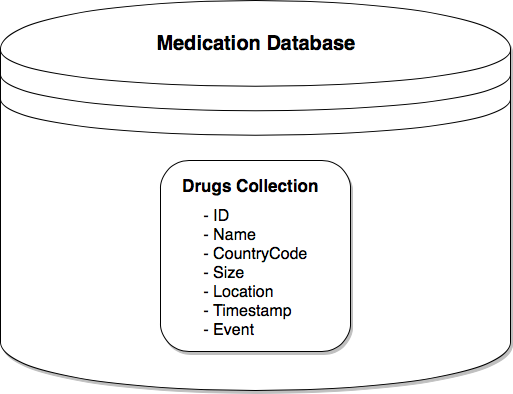
\includegraphics[width=\textwidth]{Mongo_DataModel} 
\caption{\label{fig:datamodel}Applied data model} 
\end{figure}

\subsection{Possibilities of extension}

Henrici \cite[p.121 ff.]{henrici} describes four alternative channels to authenticate and authorized the right tags and to prevent attacks on RFID applications. 
The first possibility of an alternative channel is to use written text to authenticate special operations, for instance on packaging. The master key can be printed on the interior of the product package and is proposed as key recovery mechanism.
Furthermore, optical barcodes can be used together with RFID to ensure identification of items. Especially barcodes attached to each item can be used for general identification of objects. Additionally, RFID tags might be used to assign items of high value.
A third possibility of using side channels is to use optical input, such as photodiodes attached to RFID tags. Each RFID tag can use flashes of light (also called optical channel) to transfer data.   
Lastly, a physical contact channel can also be used alternatively. Compared to smartcards, this methods defends against wireless sabotage or denial of service attacks.


















 
